\documentclass[12pt]{article}
% controlling the geometry of the page:
\usepackage[margin=1in, paperwidth=8.5in, paperheight=11in]{geometry} 
\usepackage{amsmath, amssymb} % useful math symbols and environments

% pretty colors!
\usepackage[dvipsnames]{xcolor}
\colorlet{darkgrey}{black!70}
\colorlet{darkgreen}{green!50!black}

\usepackage{graphicx} % for inserting figures with \includegraphics
\usepackage{setspace} % for controlling space between lines, paragraphs, etc.

\usepackage{tikz} % for drawing diagrams
\usetikzlibrary{arrows,automata,positioning} 
\usetikzlibrary{decorations.markings}
\usetikzlibrary{decorations.pathreplacing}
\usetikzlibrary{patterns}
\usetikzlibrary{shapes.geometric}

\usepackage{fancyhdr} % for controlling headers and footers
\usepackage{newtx} % changes the default font family
\usepackage{enumitem} % controllable labels for ordered and unordered lists

\usepackage{hyperref} % controls hyperlinks, both internal and external
\hypersetup{
    colorlinks=true,
    urlcolor=blue,
}

\setlength{\headheight}{14.5pt}
\newcommand{\Q}{\mathbb{Q}}
\newcommand{\R}{\mathbb{R}}
\newcommand{\Z}{\mathbb{Z}}
\DeclareMathOperator\Rect{\mathbf{Rect}}
\DeclareMathOperator\Tri{\mathbf{Tri}}
\DeclareMathOperator\Sq{\mathbf{Sq}}
\DeclareMathOperator\Light{\mathbf{Light}}

\newenvironment{red}{\color{red}}{\ignorespacesafterend}

% I don't like how LaTeX renders section headings by default
\renewcommand{\section}[1]{\begin{center} \textbf{#1} \\\end{center}}
%
\setlength{\parindent}{0in}
%\oddsidemargin=-.25in
\allowdisplaybreaks
\pagestyle{fancy}
\renewcommand{\headrulewidth}{0pt}
\lhead{MATH 312}
\rhead{Spring 2025}
%\lfoot{\copyright\ CLEAR Calculus 2010}
\cfoot{}
\renewcommand{\thefootnote}{*} 
\hyphenpenalty=10000 % LaTeX by default really likes hyphenating things

% all the stuff above this line is called the preamble...
%##################################################################
\begin{document} % this is always the first line of what's actually produced
\section{Homework \#1} % notice that if you want the character # to appear, you have to "escape" it with a backslash

Here's your homework for this week, due Sunday 1/26 by pdf upload to Canvas. I'm also posting the .tex source on my \href{https://github.com/rhinopotamus/math312}{new MATH 312 github repo}, with lots of comments, so that you can see how it is made and borrow some tricks.

\begin{enumerate} % enumerate produces ordered lists! by default they are made with number labels.
    \item In class on Wednesday we discussed an attendance and participation policy. I think we settled on a coherent vision of a respectful and involved classroom community, and in particular, we talked about when it's okay and not okay to be absent. Please write an appropriate amount of words about what you understand the attendance and participation policy to be.

    \item Get set up with a mathematical document typesetting system. Refer to this \href{https://github.com/rhinopotamus/math312/blob/main/resources/typesetting.md}{typesetting resources document} for some pointers.

    \item In class on Wednesday, we explored the group of symmetries of a rectangle, which I shall call $\Rect$. Explore $\Sq$, the group of symmetries of a square.
    \begin{itemize} % itemize produces unordered lists!
        \item We decided that $\Rect$ contains 4 distinct symmetries (and we say that $\Rect$ has \textit{order} 4 and write $|\Rect| = 4$):
        \begin{itemize} % you can nest lists pretty much as deeply as you want :)
            % notice that letters that I intend as math are wrapped in math-mode indicators $..$ or \( .. \)
            \item $e$, the ``identity'' symmetry where you do nothing
            % notice how quotes are made: that's two backticks for an opening quote and two apostrophes for a closing quote
            \item \(f\), a (vertical) flip
            \item $s$, a (horizontal) spin
            \item $r$, a half-turn rotation (so it doesn't matter whether it's cw or ccw)
        \end{itemize}
        Certainly $|\Sq| > |\Rect|$ -- in particular, a quarter-turn rotation is a symmetry of the square that isn't a symmetry of a rectangle. How many \textit{distinct} symmetries are in $\Sq$? Give them good letter names.
        \item Here's the Cayley diagram for $\Rect$:

% This is an example of a diagram generated with Tikz code. I have stolen some tricks from Dana Ernst to get started.

% This is some stuff to setup some different color arrow styles.
% The magic word "stealth" has to do with the arrow tips.
\tikzstyle{b} = [draw, very thick, blue, stealth-stealth]
\tikzstyle{r} = [draw, very thick, red, stealth-stealth]
\tikzstyle{g} = [draw, very thick, PineGreen, stealth-stealth]
\tikzstyle{p} = [draw, very thick, Orchid, -stealth]

% The figure environment lets you put captions and labels on things.
% If you use an editor with code-folding, it is also helpful for folding up the entire figure so you don't have to scroll back and forth across it every time.
\begin{figure}[!ht] 
\centering
\begin{tikzpicture}[scale=1.5,auto]
\node (e) at (-2,1) {
    \begin{tikzpicture}[every node/.style={minimum size=.65cm}]
        \node [draw] (1) {$1$};
        \node [draw, right=0cm of 1] (2) {$2$};
        \node [draw, below=0cm of 2] (3) {$3$};
        \node [draw, left=0cm of 3] (4) {$4$};
    \end{tikzpicture}
};
\node (s) at (2,1) {
    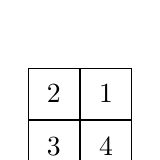
\begin{tikzpicture}[every node/.style={minimum size=.65cm}]
        \node [draw] (2) {$2$};
        \node [draw, right=0cm of 2] (1) {$1$};
        \node [draw, below=0cm of 1] (4) {$4$};
        \node [draw, left=0cm of 4] (3) {$3$};
    \end{tikzpicture}
};
\node (r) at (2,-1) {
    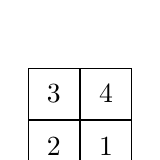
\begin{tikzpicture}[every node/.style={minimum size=.65cm}]
        \node [draw] (1) {$1$};
        \node [draw, left=0cm of 1] (2) {$2$};
        \node [draw, above left = 0cm of 1] (3) {$3$};
        \node [draw, above=0cm of 1] (4) {$4$};
    \end{tikzpicture}
};
\node (f) at (-2,-1) {
    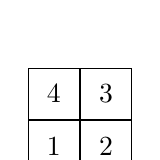
\begin{tikzpicture}[every node/.style={minimum size=.65cm}]
        \node [draw] (1) {$1$};
        \node [draw, right=0cm of 1] (2) {$2$};
        \node [draw, above right = 0cm of 1] (3) {$3$};
        \node [draw, above=0cm of 1] (4) {$4$};
    \end{tikzpicture}
};
\path[b] (e) to node {$s$} (s);
\path[b] (f) to node {$s$} (r);
\path[r] (e) to node [left] {$f$} (f);
\path[r] (s) to node {$f$} (r);
\path[g] (e) to node [pos = 0.2, below] {$r$} (r);
\path[g] (f) to node [pos = 0.8, below] {$r$} (s);
\path[p] (e) to[loop left] node {$e$} (e);
\path[p] (f) to[loop left] node {$e$} (f);
\path[p] (s) to[loop right] node{$e$} (s);
\path[p] (r) to[loop right] node{$e$} (r);
\end{tikzpicture}
\caption{Cayley diagram for the group of symmetries of a rectangle.}
\label{fig:Cayley_rectangle} % Labels can help you reference figures elsewhere in a document.
\end{figure}

    Draw a Cayley diagram for $\Sq$. Notes:
    \begin{itemize}
        \item It would be reasonable to omit the identity loops to reduce visual clutter.
        \item Will all of your arrows be double-headed this time?
        \item I've generated this diagram within LaTeX using TikZ code. Feel free to modify my source to draw your own, but also feel free to hand-draw your diagram.
    \end{itemize}

    \item We decided that $\Rect$ is \textit{generated by} any two non-trivial symmetries and we wrote several different \textit{presentations}, such as $\Rect = \langle f, s \mid f^2 = s^2 = e, fs = sf \rangle$. 
    \begin{itemize}
        \item See if you can determine a minimal generating set for $\Sq$. (There are 12 possibilities.)
        \item See if you can write a presentation for $\Sq$.
    \end{itemize} 

    \item What's similar and what's different between $\Rect$ and $\Sq$?
    \begin{itemize}
        \item In $\Rect$, every pair of symmetries \textit{commuted} -- for instance, $fr = rf$. (We say that $\Rect$ is \textit{abelian}.) Is this true for $\Sq$?
        \item In $\Rect$, every symmetry was its own \textit{inverse} -- for instance, $ss \text{ (aka } s^2) = e$. (We say that every element of $\Rect$ is \textit{idempotent}.) Is this true for $\Sq$?
    \end{itemize}

    \end{itemize}
\end{enumerate}

Here are some extension problems. You should try ``some'' of them. How many is ``some''? Idk.

\begin{enumerate}[resume]
    \item Count the symmetries of every upper-case letter in the English alphabet. Assume they're the most boring, non-decorated, sans-serif versions possible; for instance, ``U'' should really look like ``$\bigcup$''. Notice that every letter has at least one symmetry (the identity).

    \item Explore $\Tri$, the group of symmetries of an equilateral triangle.

    \item Write out the multiplication table for $\Rect$. Convention: the box in the $s$ row and the $r$ column is $sr$ (not $rs$).
    % This is the other math-mode delimiter, but it's for "display math" rather than "inline math." It renders bigger and centered.
    \[
        \begin{array}{c||c|c|c|c}
              & e & s & r & f \\ \hline\hline
            e &   &   &   &   \\ \hline
            s &   &   &   &   \\ \hline
            r &   &   &   &   \\ \hline
            f &   &   &   &
        \end{array}
    \]

    \item Write out the multiplication table for $\Sq$.
    \item Write out the multiplication table for $\Tri$.

    \item Here is a thing called a \textit{frieze}. It goes on infinitely in both directions.
    \tikzstyle{up}=[shape=diamond, aspect=.5,anchor=south,fill=orange,draw]
    \tikzstyle{down}=[shape=diamond, aspect=.5,anchor=north,fill=orange,draw]
    \[
    \hspace*{-5mm}
    \scalebox{1.2}{
      \begin{tikzpicture}[scale=1.2]
        \begin{scope}[shift={(0,0)}]
          \tikzstyle{every node}=[font=\footnotesize]
          \draw (-1,0) node [down] {};
          \draw (0, 0) node [up] {};
          \draw (1, 0) node [down] {}; 
          \draw (2, 0) node [up] {};
          \draw (3, 0) node [down] {};
          \draw (4, 0) node [up] {};
          \draw (5, 0) node [down] {}; 
          \draw (6, 0) node [up] {};
          \draw (7, 0) node [down] {};
          \draw[thick] (-1.9,0) -- (7.9,0);
          \draw (-2.15,-.01) node {\small $\cdots$};
          \draw (8.21,-.01) node {\small $\cdots$};
        \end{scope}
    \end{tikzpicture}}
    \]
    Explore the group of symmetries of this figure. (Is it finite or infinte?)

    \item Not every group comes from symmetries of a geometric figure (they're just nice examples to play with). Consider two light switches on a wall side by side, and think about all the possible actions that you can do to the two light switches. For example, one action is to toggle the left light switch while leaving the right one alone. Let's call this group of actions $\Light_2$.
    \begin{enumerate}[label=\rm{(\alph*)}]
        \item How many distinct actions does $\Light_2$ have? Give these actions good letter names.
        \item Draw a Cayley diagram for $\Light_2$.
        \item Find a minimal generating set for $\Light_2$ and write a presentation.
        \item Seem familiar?
    \end{enumerate}

    
\end{enumerate}

%#################################################################
\end{document}